
\subsection{Planning Reasoning} % (ToT, ReWOO, hierarchical)


Planning is a central component of intelligent behavior, enabling agents to decompose problems, sequence decisions, and navigate complex environments with foresight. Recent research has increasingly explored planning in the context of large language models (LLMs), either as autonomous agents or as components in broader systems. In this section, we categorize existing work in agent planning for reasoning into six methodological styles, where each category highlights a distinct planning strategy that supports complex agentic reasoning. 

\begin{figure}
    \centering
    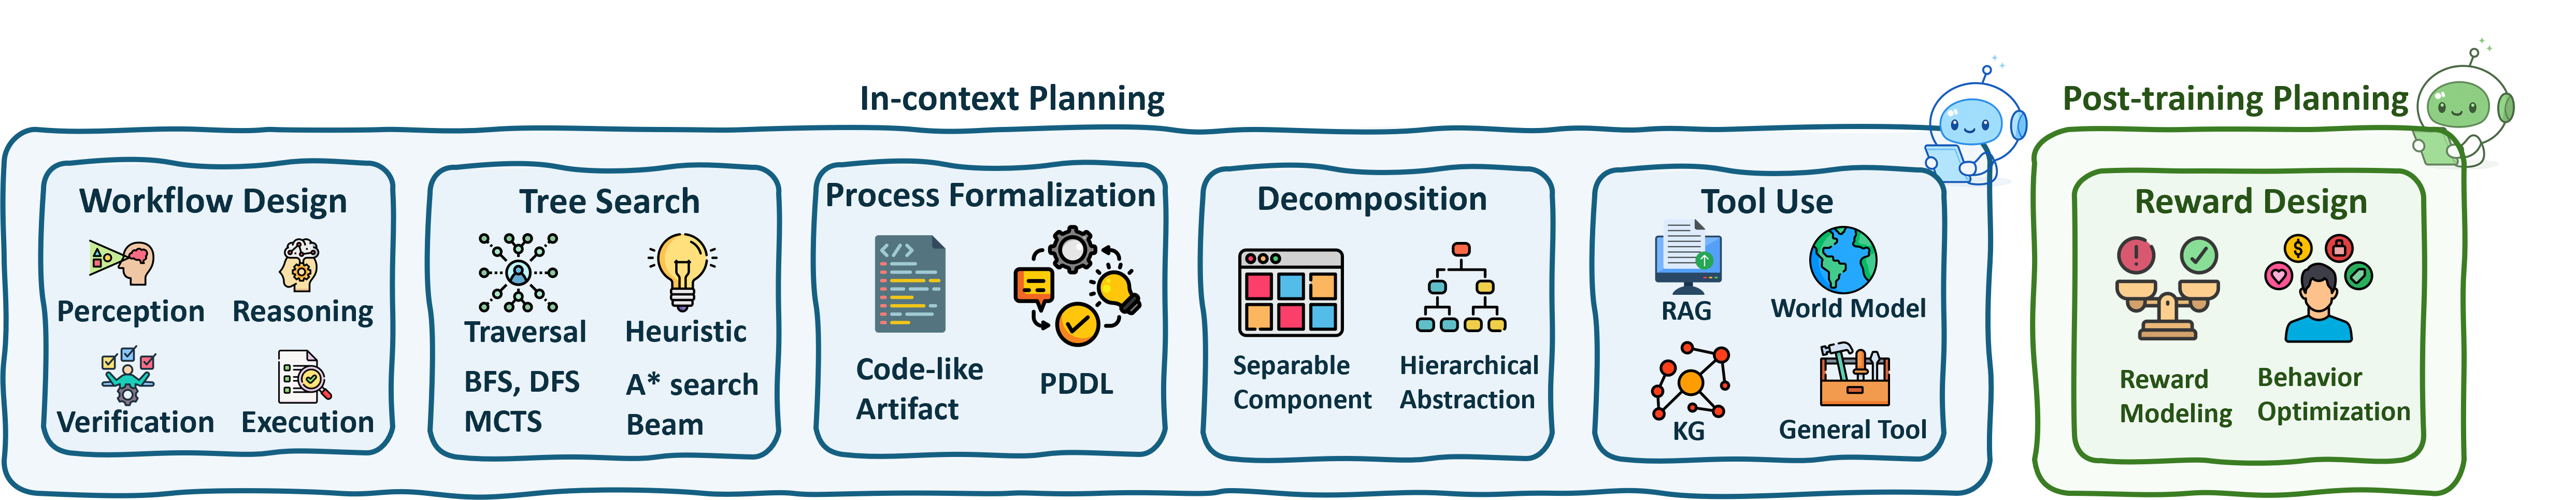
\includegraphics[width=\linewidth]{arxiv/figs/planning.png}
    \caption{Overview of \textbf{Planning Reasoning} in LLM agents, categorized into in-context planning and post-training planning.}
    \label{fig:planning}
\end{figure}

\begin{table*}[!t]
% \newcommand\TODO{\textcolor{magenta}{[TODO]}}
\centering
\caption{Representative \textbf{Agentic Planning} systems categorized by \textit{Modality}, \textit{Structure}, \textit{Format}, and \textit{Tool}.}
\renewcommand{\arraystretch}{1.15}
\setlength{\tabcolsep}{6pt}
\begin{tabular}{p{3cm}>{\centering\arraybackslash}p{3cm}>{\centering\arraybackslash}p{4cm}>{\centering\arraybackslash}p{5.5cm}}
\toprule
\textbf{Method} & \textbf{Structure} & \textbf{Format} & \textbf{Tool} \\
\midrule
\rowcolor[HTML]{F5F5F5}
\multicolumn{4}{l}{\textbf{Modality I: Language Agents (e.g., Search Agents, Code Agents)}} \\
ReWOO~\cite{xu2023rewoo} & Decomposed & Natural Language & None \\
Reflexion~\cite{shinn2023reflexion} & Sequential & Natural Language & None \\
LLM+P~\cite{liu2023llmp} & Sequential & Formal Language & None \\
IPC~\cite{valmeekam2023planning} & Sequential & Formal Language & None \\
ToT~\cite{yao2023tree} & Tree & Natural Language & None \\
GoT~\cite{besta2024graph} & Graph & Natural Language & None \\
AoT~\cite{sel2023algorithm} & Graph & Natural Language & None \\
HTP~\cite{gui2025hypertree} & Hypertree & Natural Language & Retrieval \\
RefPlan~\cite{jeong2025reflect} & Tree & Constrained Space & None \\
Gorilla~\cite{patil2024gorilla} & Sequential & Programming Language & Retrieval, API \\
CodeNav~\cite{gupta2024codenav} & Sequential & Programming Language & Code Indexer, Code Search \\
PoG~\cite{chen2024plan} & Graph & Natural Language & Knowledge Graph \\
Tool-Planner~\cite{liu2025toolplanner} & Sequential & Natural Language & Tool Cluster \\
\midrule
\rowcolor[HTML]{F5F5F5}
\multicolumn{4}{l}{\textbf{Modality II: Visual/Multimodal Agents (e.g., GUI Agents, Embodied Agents)}} \\
VisualPredictor~\cite{liang2024visualpredicator} & Tree & Formal Language & None \\
LLM-Planner~\cite{song2023llmplannerfewshotgroundedplanning} & Sequential & Formal Language & Object Detector, KNN \\
Agent-E~\cite{abuelsaad2024agent} & Sequential & Formal Language & DOM Grounder, Screenshot \\
Agent S~\cite{agashe2024agent} & Hierarchical & Natural Language & API, Search, Memory \\
ExRAP~\cite{yoo2024exploratory} & Sequential & Natural Language & Memory \\
AESOP~\cite{sinha2024real} & Reactive & Natural Language & Anomaly Detector \\
HRV~\cite{cornelio2025hierarchical} & Hierarchical & Formal Language & Symbolic Verifier \\
BehaviorGPT~\cite{zhou2024behaviorgpt} & Sequential & Visual Features & World Model \\
Dino-WM~\cite{zhou2024dino} & Tree & Visual Features & World Model \\
FLIP~\cite{gao2024flip} & Sequential & Visual Features & Language Model \\
\bottomrule
\end{tabular}
\label{tab:agentic_planning_methods}
\end{table*}

\subsubsection{In-context Planning}
\paragraph{Workflow Design.} Workflow-based approaches often emphasize structuring the overall planning process into distinct stages (e.g., perception, reasoning, execution, verification), which are either explicitly scaffolded or learned implicitly. For example, \cite{liu2023llmp,valmeekam2023planning,xu2023rewoo,hao2024llm} design planning pipelines that decompose task solving into subtasks, often leveraging a deliberate plan-and-act framework. Similarly, \cite{zhou2022least,wang2023plan,sel2023algorithm,shen2023hugginggpt} rely on structured prompting to sequentialize tasks and guide reasoning progression. Methods like \cite{liu2023plan} use structured transitions between diverse ``X-of-Thought'' strategies. PERIA \cite{ni2024peria} combines perception, imagination, and action in a unified multimodal workflow. Others such as \cite{erdogan2025plan} explicitly target long-horizon planning through structured sequencing, while \cite{wen2024codeplan} build workflows for code-related planning. 


These workflows are then grounded by a reactive controller that iteratively consumes the current state and interleaves reasoning with actions: in web automation, agents follow inspect-reason-act-observe loops \cite{yao2023react,deng2023mind2web}, with robustness improved by dynamically adapting in-context examples \cite{lutz2024wilbur}; in code, agents decide immediate executions/API calls, read outputs or errors, and refine step-by-step \cite{wang2024executable,patil2024gorilla,shinn2023reflexion,gupta2024codenav,rahman2025marco,he2024enhancing,rawat2025pre,aksitov2023rest,jiang2024self}; in robotics, monitors trigger on-the-fly safety interventions and VLM-guided subgoal execution with real-time adjustment \cite{sinha2024real,shah2023lm}. This \emph{reactive workflow} view unifies scripted stage design with online adaptation: the workflow provides interpretable structure and interfaces (what is done when), while the reactive loop supplies closed-loop grounding and error recovery (how it is done in context). The approach is broadly effective yet can accumulate errors over long horizons, motivating incremental verification and memory within the workflow to stabilize execution.


\paragraph{Tree Search / Algorithm Simulation.} Tree-based search strategies, especially BFS, DFS, A*, MCTS, and beam search, have become prominent as interpretable and effective planning scaffolds. Several works simulate tree traversal algorithms to mimic deliberative processes: \cite{yao2023tree,markowitz2024tree,long2023large,koh2024tree} apply breadth- or depth-first strategies to explore structured thought trees. A*-like guided expansions appear in \cite{wang2024qstar,meng2024llmastar,liu2024multimodal}, providing heuristic-driven planning with state evaluation. Besides that, MCTS is heavily explored in agentic research: \cite{hao2023reasoning,putta2024agent,sprueill2023monte,yu2023prompt,zhao2023large,ding2023everything,chen2024tree,kong2024latent,feng2023alphazero,yoon2025monte,schultz2024mastering,chen2025broaden} use MCTS or its variations for controlled exploration and improved reasoning fidelity. Beam search is leveraged in \cite{xie2023self,golovneva2023pathfinder,qian2025discriminator} to prune and prioritize reasoning trajectories efficiently. Other tree-search-inspired works include \cite{gandhi2024stream} which uses learned search policies and \cite{saha2024system} which differentiates between fast (reactive) and slow (deliberative) planning. These methods mirror traditional algorithmic planning, grounding LLMs' search processes in classical decision-making frameworks.

This search-over-hierarchy view maps cleanly onto domain systems. In the web setting, planner-executor architectures generate high-level subtask trees in natural language and bind leaves to DOM-grounded actions, often with memory to persist context \cite{abuelsaad2024agent,guan2023intelligent,agashe2024agent}. For code agents, hierarchical task trees and pseudo-code plans recursively break problems into compilable/editable units, while structured pipelines embed hierarchical RL or MCTS within the tree to choose promising edits and verification paths \cite{gui2025hypertree,ni2024tree,chen2025enhancing,hu2025divide,antoniades2024swe}. In robotics, behavior trees and high-level goal decomposition translate language instructions into subgoal sequences executed by low-level controllers and skills \cite{lykov2024llm,cao2023robot,izzo2024btgenbot,ahn2022icanisay,huang2022inner}. 

Taken together, hierarchical tree-search couples \emph{plan synthesis} (node expansion, heuristic/evidence-based selection) with \emph{plan realization} (leaf grounding and feedback), yielding interpretable, long-horizon agents that can backtrack, refine, and verify before committing to irreversible actions, while remaining flexible enough to incorporate learned policies and memory for efficiency and robustness.


\paragraph{Process Formalization.} Formalizing planning through symbolic representations, programming languages, or logic frameworks ensures compositionality, interpretability, and generalization. Several works encode plans as code-like artifacts or PDDL programs: \cite{guan2023leveraging,mahdavi2024leveraging,katz2024thought,wen2024codeplan,hao2024planning,vyas2024llm} incorporate symbolic logic or procedural programming into LLM prompting or output generation. These representations enable downstream tool execution and interface more cleanly with classical planners or robot controllers. PDDL-based formulations explicitly bridge LLM planning with well-established planning ecosystems, as in \cite{mahdavi2024leveraging,katz2024thought}. CodePlan \cite{wen2024codeplan} highlights the use of program synthesis to scaffold long-horizon reasoning. Such formalization provides structural scaffolds for agent behavior and often enhances explainability and robustness of the generated plans.

\paragraph{Decoupling / Decomposition.} Decoupling strategies aim to modularize complex planning into separable components such as goal recognition, memory retrieval, and plan refinement. Notably, ReWOO \cite{xu2023rewoo} explicitly separates observation and reasoning modules to optimize for efficiency. Similarly, works like \cite{zhang2025atomic, dong2024diffuserlite,lo2024goal,li2024agent,wang2023goplan,vyas2024llm,kang2025retrointext} break reasoning into reusable or hierarchical abstractions. \cite{gui2025hypertree} promotes hierarchical thinking through hypertrees, while \cite{liang2024visualpredicator} abstracts the world with symbolic predicates to reduce planning burden. Others, such as \cite{ye2024beyond} and \cite{kong2024latent}, decompose via latent variables or state spaces. These decompositions not only enhance tractability, but also align with neural-symbolic hybrid frameworks. They are especially common in long-horizon or multi-agent planning scenarios, such as \cite{zheng2024planagent,nayak2024long}.\nocite{wei2024robust,bao2025latte,chen2024wapiti,liu2025breaking,liu2024logic,liu2024class,liu2024aim,liu2023topological,zeng2025pave,zeng2024graph,lin2025moralise,lin2024backtime,qiu2025saffron,qiu2025ask,qiu2025efficient,qiu2024tucket,qiu2023reconstructing,qiu2022dimes,xu2024discrete,li2025model,zou2025transformer,qiu2024gradient,yoo2025embracing,yoo2025generalizable,yoo2024ensuring,chan2024group,wu2024fair,he2024sensitivity,wang2023networked}

\paragraph{External Aid / Tool Use.} Many systems leverage external structures or tools to aid planning, including retrieval-augmented generation (RAG), knowledge graphs, world models, and general-purpose tool use. Knowledge-augmented frameworks like \cite{chen2024plan,cornelio2025hierarchical,meng2025telograf,zhong2024flexplanner, zhang2025atomic} inject structured representations (e.g., graphs, scene layouts) into the LLM context. RAG-style systems \cite{yoo2024exploratory,li2024benchmarking, zou2025gtr} retrieve relevant knowledge to support continual instruction planning. World model-based agents such as \cite{hao2023reasoning,guan2023leveraging,qiao2024agent,zhou2024behaviorgpt,zhou2024dino,gao2024flip,liu2025continual,wang2025adawm} learn or leverage environment models for model-based planning. Tool-oriented frameworks like HuggingGPT \cite{shen2023hugginggpt}, Tool-Planner \cite{liu2025toolplanner}, and RetroInText \cite{kang2025retrointext} use external APIs or modular toolchains to support planning execution. These systems often reflect agent-environment interaction and capitalize on external resources to scaffold or augment LLM capabilities.

\subsubsection{Post-training Planning}


\paragraph{Reward Design / Optimal Control.} Finally, planning as optimization entails designing suitable reward structures and solving for optimal behavior using RL or control-theoretic tools. Reflexion \cite{shinn2023reflexion}, Reflect-then-Plan \cite{jeong2025reflect}, and Rational Decision Agents \cite{ye2023rational} incorporate utility-based learning to guide planning behavior. Reward modeling appears in works such as \cite{chen2025scaling}, while others like \cite{luyten2025strategic} emphasize reward shaping. Optimal control is tackled explicitly in \cite{ma2024non,ni2025physics,matada2024generalizable, su2025toolorchestra}, and trajectory optimization via diffusion models is seen in \cite{xie2025latent,xiao2023safediffuser,shan2025contradiff}. Offline RL methods like \cite{kong2024latent,ruoss2024amortized,wang2023goplan} leverage pretrained dynamics or cost models. The control-theoretic orientation in these works complements symbolic or heuristic approaches by optimizing over continuous, structured, or learned reward spaces.

%%%%%%%%%